\documentclass{article}

\usepackage{fullpage}
\usepackage{amsmath}
\usepackage{amssymb}
\usepackage{graphicx}
\usepackage{multirow}

% Schreibweisen für bestimmte Überschriften:
%
%					Beispiele
% \section{große Überschrift} 		Folgen und Reihen
% \subsection{große Überschrift} 	Häufungspunkte und Grenzwerte von Folgen
% \paragraph{Definition}
% \paragraph{Schreibweise}
% \paragraph{Bemerkung}
% \paragraph{Bezeichnung}
% \paragraph{Satz}

\begin{document}

% zwischen den beiden folgenden kommentaren schreiben

% start

\subsection{Arcus Funktionen\newline}

% arcsin Function
\paragraph{Arcsin}
\begin{tabular}{ l l }
\multirow{3}{*}{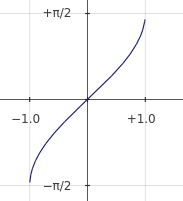
\includegraphics[scale=0.5]{png/arcsin.png}} & \\ \\
 & $ arcsin : [-1, 1] \to \left[-\frac{\pi}{2}, \frac{\pi}{2}\right] $ \\ \\
 & $ arcsin(x), |x|<1 $ \\ \\
 & $ arcsin'(x) = \frac{1}{\sqrt{1-x^2}} $ \\ \\ \\
\hline
\end{tabular}

\vspace{2ex}

% arccos Function
\paragraph{Arccos}
\begin{tabular}{ l l }
\multirow{3}{*}{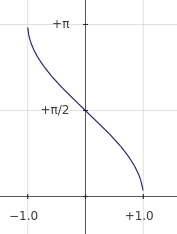
\includegraphics[scale=0.5]{png/arccos.png}} & \\ \\
 & $ arccos : [-1, 1] \to [0, \pi] $ \\ \\
 & $ arccos (x), |x|<1 $ \\ \\
 & $ arccos'(x) = -\frac{1}{\sqrt{1-x^2}} $ \\ \\ \\ \\
\hline
\end{tabular}

\vspace{2ex}

% arctan Function
\paragraph{Arctan}
\begin{tabular}{ l l }
\multirow{3}{*}{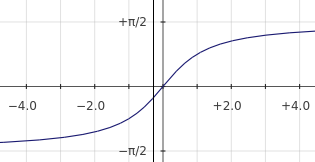
\includegraphics[scale=0.5]{png/arctan.png}} & \\ \\
 & $ y = arctan(x) $ \\ \\
 & $ arctan : \mathbb{R} \to \big(-\frac{\pi}{2}, \frac{\pi}{2}\big) $ \\ \\
 & $ arctan'(x) = \frac{1}{1+x^2} $ \\ \\
\hline
\end{tabular}

\vspace{2ex}

% arccot Function
\paragraph{Arccot}
\begin{tabular}{ l l }
\multirow{3}{*}{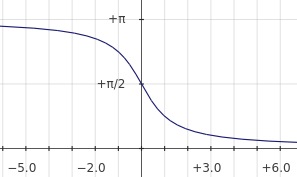
\includegraphics[scale=0.5]{png/arccot.png}} & \\ \\
 & $ y = arccot (x) $ \\ \\
 & $ arccot : \mathbb{R} \to \big(0, \pi \big)$ \\ \\
 & $ arccot'(x) = -\frac{1}{1+x^2} $ \\ \\
\hline
\end{tabular}

\newpage
\subsection{Hyperbelfunktionen\newline}

\begin{tabular}{ l l }
\multirow{3}{*}{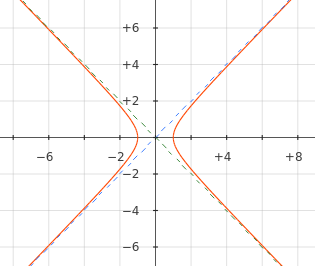
\includegraphics[scale=0.5]{png/hyperbelfunc.png}} & \\ \\
 & $ Hyperbelgleichung : x^2 - y^2 = 1 $ \\ \\
 & $ y^2 = x^2 - 1 $ \\ \\
 & $ y = \sqrt{x^2 - 1} $ \\ \\ \\ \\ \\ \\ \\
\hline
\end{tabular}

\vspace{4ex}

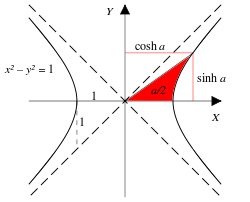
\includegraphics[scale=0.5]{png/cosh.png}
\[ x = cosh(t) = \frac{1}{2}\left(\mathrm{e}^t + \mathrm{e}^{-t}\right) \]
\[ y = sinh(t) = \frac{1}{2}\left(\mathrm{e}^t - \mathrm{e}^{-t}\right) \]
$(x,y)$ liegt auf der Hyperbel, weil
\[ x^2 - y^2 = cosh^2t - sinh^2t = \frac{1}{4} \left(\left(\mathrm{e}^t+\mathrm{e}^{-t}\right)^2 - \left(\mathrm{e}^t+\mathrm{e}^{-t}\right)^2\right) \]
\[ = \frac{1}{4}\left(\mathrm{e}^{2t}+2+\mathrm{e}^{-2t} - \left(\mathrm{e}^{2t}-2+\mathrm{e}^{-2t}\right)\right) = 1 \]

\vspace{5ex}
\subsection{Tangens Hyperbolicus und Kotangens Hyperbolicus\newline}

\[ tanh(t) = \frac{sinh(t)}{cosh(t)} = \frac{\mathrm{e}^t - \mathrm{e}^{-t}}{\mathrm{e}^t + \mathrm{e}^{-t}} = \frac{\mathrm{e}^{2t} - 1}{\mathrm{e}^{2t} + 1} \]
\[ coth(t) = \frac{1}{tanh(t)} = \frac{\mathrm{e}^{2t} + 1}{\mathrm{e}^{2t} - 1} \]
% stop

\end{document}
